%-----------------------------------------------------------------------------
%	Capitulo N
%-----------------------------------------------------------------------------

%borrar esta sección si no hace nada 
%\lhead[\thepage]{CAPÍTULO \thechapter. \rightmark}
%\rhead[CAPÍTULO \thechapter. \leftmark]{\thepage}
%borrar esta sección si no hace nada 

%Nombre del Capitulo
\chapter{Marco Teórico}
\markboth{Marco Teórico}{Marco Teórico}
%Faltan secciones aqui
%Sección
\section{Ciencia de Datos}
\lhead[\thepage]{\thesection Ciencia de Datos}

\subsection{Definición}

La Ciencia de Datos es el estudio del origen de la información, que representa  y como puede convertirse en un recurso valioso en los planes estratégicos de las organizaciones.\cite{1rouse}

Se considera una etapa evolutiva, dada por la unión de varios campos interdisciplinarios como la inteligencia de negocios, el modelado estadístico y las matemáticas.\cite{2whatisdatasc}Tambien comprende área tales como: minería de texto, computación paralela y distribuida, \emph{machine learning}, bases de datos NoSQL, herramientas para visualización, entre otras.

En la actualidad se enfoca fuertemente en el área de \emph{Big Data} donde es necesario el trabajo conjunto de diversas áreas para poder llevar a cabo procesos de análisis, para trabajar con cantidades masivas de datos.

\subsection{Rol del Científico de Datos}

El científico de datos, es aquel que obtiene conocimiento a partir de un conjunto de datos para responder a preguntas que se le han formulado.\cite{5pellicer} Generalmente posee gran experiencia y un alto grado de conocimiento en una de las áreas interdisciplinarias de la ciencia de datos y un conocimiento avanzado en algunas de las otras que conforman esta disciplina. 

Es considerado como un nuevo perfil profesional, evolución del analista de negocio o analista de datos \cite{3carbo,4uespana,5pellicer}. Aunque su enfoque sobrepasa al de la inteligencia de negocios, se adentra en la exploración y análisis de datos de múltiples fuentes y formatos, buscando las soluciones de mayor valor para la organización \cite{5pellicer}.
 El papel del científico de datos es variado, en el mercado laboral de la industria de ciencia de datos surgen distintos roles dependientes de aspectos como, las herramientas o tecnologías que deben manejarse en el área, habilidades o técnicas  utilizadas al abordar un problema. Para poder manejar estos aspectos un cientifico de datos debe tener una formación solida en ciencias de la computación y aplicaciones, modelado, estadísticas, análisis y matemáticas \cite{5pellicer}.

 \begin{figure}[!htbp]
    \centering
    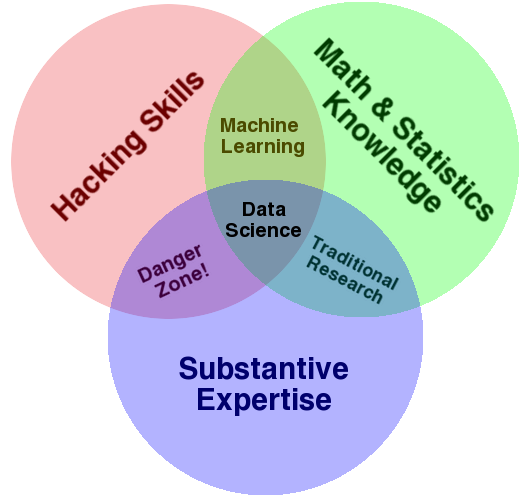
\includegraphics[width=0.7\textwidth]{Figuras/Data_Science_VD.png}
    \caption{Diagrama de Ven, habilidades del científico de datos}
    \label{fig:vennskills}
    \source{http://drewconway.com/zia/2013/3/26/the-data-science-venn-diagram}
\end{figure}

 Debido a la variedad de roles que debe cumplir un científico de datos, el trabajo en ciencia de datos no es realizado por un único individuo. La tendencia es crear equipos multidisciplinarios donde aquellos que los componen (científicos de datos) ocupan distintos roles con una especialidad y función en concreto (como se ejemplifica en la Figura \ref{fig:vennskills}), pero con nociones esenciales de las funciones de los otros miembros del equipo \cite{5pellicer}.

\subsection{Grandes Volúmenes de Datos (\emph{Big Data})}

\subsubsection{Definición}

EL termino grandes volúmenes de datos (conocido en el ámbito comercial como \emph{Big Data}), se refiere a cantidades masivas de datos (tanto estructurados, no estructurados y semi-estructurados), que superan la capacidad de las bases de datos relacionales convencionales para poder ser almacenados, administrados y procesados en un tiempo  aceptable \cite{7sasinc}.

El crecimiento contante de los volúmenes de datos requiere de tecnologías rentables, y eficientes en el manejo del tiempo, que puedan ser usadas para generar conocimiento de valor para la toma de decisiones \cite{8gartner,9ibm}.

 
El ``Modelo de las 3 V's" de Doug Laney \cite{10laney}, recoge las definiciones de tres aspectos fundamentales de los datos, que para el 2001 eran manejados en el área de \emph{E-commerce} o comercio electrónico, sin embargo el modelo planteado por Laney sirvió de punto de apoyo en los inicios de \emph{Big Data}. Estos atributos claves son : volumen, velocidad y variedad.

\begin{itemize}
\item Volumen:  se refiere a la vasta cantidad de datos que se generan cada segundo. Estos volúmenes de datos que aumentan constantemente, hacen que su almacenamiento y análisis imposible usando tecnologías tradicionales de base de datos. La tecnología usada en el área de Big Data se enfoca en solucionar este problema utilizando sistemas distribuidos, donde partes de los datos son almacenados en diferentes locaciones, conectadas a  través de redes y utilizadas como un solo sistema \cite{13bernard}.

\item Velocidad: hace referencia a la velocidad a la que se generan, transmiten, procesan y almacenan nuevos datos. El incremento de este atributos en el ámbito de la generación y transmisión de datos a contribuido con la existencia de Big Data, mientras que el aumento en la velocidad de procesamiento, almacenamiento y también transmisión han sido esenciales para su análisis, lo que ha permito dar respuestas de forma más rápida a las necesidades especificas de cada negocio\cite{11pragsis}. 

  \begin{itemize}
  \item Viscocidad: atributo asociado con el retardo o latencia del tiempo de alguno de los eventos asociados a la velocidad \cite{16}. 
  \item Viralidad: atributo que describe la velocidad con la que los datos se propagan, la frecuencia con la que son recuperados y repetidos entre usuarios o eventos \cite{16}.
  \end{itemize}
 \item Variedad: se refiere a los diferentes tipos de datos que sirven de fuente, estos datos pueden venir de archivos de texto plano, correos electrónicos, fotos, vídeos, logs de transacciones, redes sociales, paginas web, entre otros \cite{13bernard}. Esta variedad no solo aplica al medio de donde proviene también a su tipo de estructura (estructurados, semi estructurados, no-estructurados). 
 
\end{itemize}

Existen nuevos modelos que surgen de la evaluación del área de \emph{Big Data} y su constante evolución, acontinuacion se definen estas nuevas variables que se incorporan a \emph{Big Data}:

 \begin{itemize}
 \item Valor: este atributo busca ponderar la utilidad de la información que puede ser obtenida de los datos. Un error común y fácil de cometes es la toma de iniciativas de grandes volúmenes de datos sin una clara comprensión del valor de negocio que traerá, esta variable es de gran importancia para medir si vale la pena comenzar un proceso de análisis de \emph{Big Data}. Ciertos autores afirman que ésta variable no depende de si se trabaja con grandes volúmenes de datos o no, puesto a que es un indicador clave en cualquier proceso de análisis \cite{16}.
 
\item Veracidad: nivel de certidumbre de los datos. Debido a la variedad de los datos, la calidad y precisión de los mismos es más difícil de controlar. Los volúmenes a menudo compensan la falta de calidad o exactitud, a partir de la cual cobra importancia la variable del valor \cite{13bernard}. La tarea de verificar la veracidad de los datos es compleja, es necesario evaluar el contexto de los datos teniendo en cuenta su procedencia, la comprensión de los mismos es importante para su utilización \cite
{18}. El científicos de datos emplean hasta un 80\% de su tiempo, en la limpieza y pre-procesamiento de los datos para asegurar un indice alto de veracidad.

\item Variabilidad: hace referencia a los cambios constante en los datos. La naturaleza de los datos no siempre es estáticas y su significado podría variar mucho en su contexto \cite{15}.

\item Visualización: atributo asociado a la representacion dada de forma visual a los datos ya procesados para su fácil entendimiento. La visualización de grandes volúmenes de datos pueden contener decenas de variables y parámetros, lo que resulta en un reto para \emph{Big Data} el como presentar estos \cite{15}. La visualización es fundamental al ser esta la manera en como se harán accesibles los datos procesados para las organizaciones. Otro aspecto a tomar en cuenta de la visualización es cuando esta variable forma parte del proceso de análisis a través de la exploración visual de datos, que puede servir como herramienta al científico de datos, la visualización de datos ayudará a los científicos a comprender qué técnicas podrían ser mejor utilizados para descubrir ideas o patrones ocultos y les ayudará a entender los resultados de la aplicación de estas técnicas, lo que ayuda a guiar el proceso de análisis de los resultados deseados \cite{17}.

\item Validez: la validez de los datos es esencial para la toma de decisiones, debido a que usar datos de fuentes  no confiables puede llevar el proceso de análisis por una ruta errónea. Los datos de entrada válidos, seguido por el procesamiento correcto de los mismos, deben dar resultados exactos.

\item Volatilidad: se refiere al tiempo en el cual los datos son válidos y por cuanto tiempo deben almacenarse, debido al factor de la variabilidad la utilidad de los datos puede cambiar, será necesario determinar en qué momento dichos datos ya no serán relevantes para el análisis actual \cite{14}.

\item Vialidad: es descrita como una cuidadosa selección de los atributos en los datos que tienen más probabilidades de predecir los resultados de mayor importancia para las organizaciones \cite{18}. Mientras que se considera que tan solo el 5\% de los atributos en los datos son responsables del 95\% de los beneficios, por lo que se debe de considerar esta cualidad\cite{19}, otros autores consideran que la vialidad no es una propiedad propia de \emph{Big Data}, sino que es una cualidad que se determina mediante el análisis de los grandes volúmenes de datos  \cite{18}.

 \end{itemize}
 
 
% \subsection{Campos Donde es Utilizado}

% 	Las posibilidades de la Ciencia de Datos y \emph{Big Data} son inmensas, existen una gran cantidad sectores que se benefician de este nuevo paradigma, afecta a las organizaciones de prácticamente cualquier industria \cite{7sasinc}:

% \begin{itemize}
% \item Ciencias Sociales: Redes sociales como Facebook o Twitter, generan millones de datos diariamente \cite{https://www.gwava.com/blog/internet-data-created-daily}, dicha data es ahora aprovechable gracias a la capacidad y enfoque que tienen las herramientas y tecnologias que han surgido para el manejo de \emph{Big Data}.

% \item Ciencias Económicas: sistemas de recomendaciones implementados por Amazon o Netflix son claros ejemplos de cómo los grandes volúmenes de datos han sido aprovechados para ayudar a entender y servir mejor a los clientes.

% \item Medicina: las agencias gubernamentales pueden ahora predecir brotes de enfermedades y hacer seguimientos en tiempo real, para que las compañías farmacéuticas puedan acelerar el desarrollo de los fármacos necesarios. Recientemente Google estudiaba implementar un algoritmo para predecir la propagación del Zika en el mundo y poder ayudar a destinar ayudas humanitarias por parte de los Gobiernos [21].

% \item Gobierno: las agencias gubernamentales son capaces de aprovechar los grandes volúmenes de datos para ayudar a los servicios públicos a afrontar mejor sus retos, frente a congestiones de tráfico, prevención de la delincuencia. frustrar ataques terroristas, detectar delitos cibernéticos, entre otros. Otras entidades como la Organización de las Naciones Unidas han destinado presupuestos para el financiamiento de proyectos de ayuda humanitaria y tratamiento del medio ambiente, como es el caso del Pulso Global.

% \item Deportes: distintos dispositivos y sensores que permiten el análisis de datos en tiempo real por medio del Internet de las Cosas, ha permitido mejorar el rendimiento de los deportistas, siendo equipos como el Real Madrid, la selección oficial de fútbol Alemana en el Mundial de Brasil 2014, escuderías de la fórmula uno como la McLaren, entre otros participantes de éste tipo de avances.

% \item Educación: el análisis de los grandes volúmenes de datos permite a los educadores tener una visión del progreso de los estudiantes, pudiendo implementar sistemas para la evaluación y mejora en el rendimiento de los mismos.

% \end{itemize}


% La ciencia de datos ofrece por tanto, nuevos y potentes enfoques para hacer descubrimientos, mediante la combinación de los campos de la estadística, computación y matemáticas, pudiendo convertir enormes flujos de datos en nuevas ideas y conocimientos [2].

%Sección
\section{Computación Distribuida}
\lhead[\thepage]{\thesection Computación Distribuida}


\subsection{Definición}

Modelo de computación caracterizado por la intervención de un grupo de sistemas independientes que bien pueden estar separados de forma física o no, sin embargo, se encuentran conectados entre sí por una red de comunicaciones, que tiene como propósito dividir una tarea en partes pequeñas que se unen para obtener un resultado final. Este tipo de sistemas, suelen estar conformados por computadores que tienen un hardware y un software independiente, a pesar de que son percibidos por el usuario como un solo sistema, del cual se puede acceder a cuyos recursos como se accede a los propios; además, este modelo también se caracteriza por su disponibilidad, puesto que en caso de que un nodo de la red falle, los servicios que correspondían a este se distribuyen en los nodos restantes \cite{47dd}.

Gracias a estos sistemas, se hace posible que instituciones de pocos recursos puedan tener acceso remoto a sus recursos computacionales, así como también que empresas pequeñas unan sus recursos para obtener uno de más fortaleza.


\subsection{El Teorema CAP}

El teorema CAP fue enunciado por Eric Brewer inicialmente como una conjetura en el año 2000 y probado formalmente en el 2002 por Seth Gilbert y Nancy Lynch en \cite{brewer}. 
En dicha conjetura Brewer afirmo que existen tres requerimientos sistemáticos esenciales relacionados de forma especial cuando se trata el diseño e implementación de aplicaciones en un entorno distribuido, dichos requerimientos son Consistencia, Disponibilidad y Tolerancia a partición, dándole el nombre CAP por sus siglas en ingles (\emph{Consistency, Availability, Partition Tolerance}).\cite{capt}

\begin{itemize}
\item Consistencia:  Un servicio es consistente si opera de forma completa o no lo hace en absoluto. Gilbert y Lynch usan la palabara atómico, en ves de consistente para evitar confusiones con la definición de consistencia en el principio ACID de sistemas de bases de datos.\cite{capt}

\item Disponibilidad: Existe disponibilidad cuando se puede acceder al servicio.\cite{capt}

\item Tolerancia a partición: ningún error que no sea la falla total de la red, tiene permitido causar que el sistema responda de forma incorrecta.\cite{capt}

\end{itemize}
	El teorema indica que garantizar dos de los requerimiento antes mencionados deriva en la deficiencia de el tercero.\cite{capt}


\subsection{Cluster}

Conjunto de nodos interconectados con dispositivos de alta velocidad, actúan en conjunto empleando el poder de cómputo de varios CPU para lograr la realización de tareas que requieran un alto rendimiento. La importancia de los cluster radica en que aumentan la disponibilidad, la fiabilidad y la escalabilidad de la red dentro del entorno distribuido. En efecto, los llamados super computadores están compuestos por un cluster que une varios computadores.\cite{46dd}

\subsection{Escalabilidad}

Constituye una propiedad de un sistema determinada por su habilidad de aumentar su capacidad de trabajo, logrando reaccionar y adaptarse a nuevas demandas sin perder la calidad y la fluidez de los servicios que ofrece. El aumento de dicha capacidad puede ser reflejado en el número de usuarios, cantidad de datos procesados o solicitudes recibidas. Se pueden describir dos tipos de escalabilidad: La horizontal y la vertical.\cite{48dd}

\subsubsection{Horizontal}

El rendimiento del sistema mejora cuando se añaden más nodos a este, implica un aumento en la capacidad, más no necesariamente en la potencia. El efecto de este tipo de escalabilidad viene dado por la posibilidad de distribuir la carga de procesamiento entre varios servidores, de esta forma, la escalabilidad permanece disponible para el usuario aunque alguno de los servidores falle. A diferencia de la escalabilidad vertical, no se ve limitada por el hardware, pues cada servidor añadido proporciona una mejora casi lineal. \cite{49dd}

\subsubsection{Vertical}

El sistema mejora en conjunto al añadir más recursos a un nodo en particular, su objetivo es hallar un mejor software, más rápido y más costoso. Se ve limitada por la capacidad del hardware, puesto que requiere agregar más memoria o procesadores más eficientes, lo cual implica en ocasiones migrar a un equipo de mayor potencia.\cite{49dd}

\subsection{Grid/Malla}

Es una tecnología que permite la utilización coordinada y concurrente de recursos heterogéneos, autónomos y distribuidos que no están sujetos a un control centralizado, por lo cual, pueden pertenecer a distintas organizaciones y encontrarse interconectados (Como sucede con el internet), permitiendo a estas mantener sus políticas de seguridad y gestión de recursos, por tanto, la tecnología empleada en la construcción de un Grid es complementaria a otras tecnologías.\cite{50dd}

Entre los principales objetivos de un grid se hallan la optimización e integración del uso de recursos distribuidos de cálculo intensivo y de grandes bases de datos, a través de middleware, emulando así la función de un cluster.\cite{50dd}

Una de las ventajas de la tecnología Grid es la facilidad que posee en cuanto a términos de escalabilidad, puesto que ello le permite crecer según las necesidades de la organización, es por ello que fueron concebidos como la creación de una red mundial de laboratorios proveedores de poder de cómputo y capacidad de almacenamiento. Un ejemplo actual de este concepto se halla en el big data, a través de los smart grids y su relación con el internet de las cosas.\cite{50dd}

\subsection{Base de datos distribuida}

Es un conjunto de múltiples bases de datos relacionadas lógicamente y distribuidas entre diferentes sitios que se interconectan a través de una red de comunicaciones. Estas bases de datos cuentan con la capacidad de realizar procesamiento autónomo, por lo cual puede realizar operaciones localizadas o distribuidas.\cite{51dd}


\subsubsection{Sistema manejador de base de datos distribuidas}

Se refiere al software que permite la gestión de una base de datos distribuida, proporcionando un mecanismo de acceso que hace que la distribución sea transparente para el usuario, es decir, este tendrá una visión de la aplicación como si se ejecutara en una sola máquina.\cite{51dd}

\subsubsection{Sistema de base de datos distribuida}

Sistema constituido por múltiples sitios de bases de datos distribuidas que se interconectan a través de un sistema de comunicaciones, puede ser definido también como el resultado de la integración entre una base de datos distribuida y el sistema de manejo correspondiente.\cite{51dd}

\subsubsection{Distribución de los datos}

Hace referencia al esquema de almacenamiento de datos empleado y el posicionamiento de estos en el sistema. Puede identificarse con cuatro tipos descritos a continuación:
\begin{itemize}
\item Centralizada: La base de datos se encuentra centralizada en un lugar, mientras que el procesamiento de datos y los usuarios se encuentran distribuidos.\cite{51dd}
\item Particionamiento o Fragmentación: Se refiere a la partición de la información para distribuir los fragmentos a diferentes sitios de la red, por tanto, cada nodo debe contener uno  o más fragmentos disjuntos de la base de datos. El objetivo final es hallar un nivel de fragmentación adecuado. Puede darse a su vez de 3 maneras: Horizontal (Se particiona una relación sobre sus tuplas o registros, cada fragmento representa un subconjunto de tuplas de la relación global), Vertical (Se particiona una relación en base a sus atributos, la clave primaria de la relación se incluye en cada fragmento)  y Mixta o Híbrida (Se aplica la fragmentación vertical seguida de la horizontal o viceversa).\cite{51dd}
\item Replicación: La información almacenada en un nodo puede o  no estar replicada en otro, otorga a la base de datos cierta tolerancia a las fallas, puesto que en caso de que algún nodo falle, la información requerida se puede hallar en otro, evitando que el funcionamiento del sistema sea centralizado. Las replicaciones pueden ser parcial (Cada fragmento está replicado en algún sitio) o total (Cada nodo alberga toda la información). Esta modalidad es útil cuando el número de consultas de solo lectura supera al de solo escritura.\cite{51dd}

\item Híbrida: Combina los esquemas de replicación y partición, se particiona una relación y a su vez, los fragmentos obtenidos se replican selectivamente.\cite{51dd}
\end{itemize} 

\section{Hadoop y Spark}

\subsection{Hadoop}

\textit{Apache Hadoop software library} es un \textit{framework} que permite el procesamiento de grandes volúmenes de datos a través de \textit{clusters} de computadoras usando un modelo de programación simple.Esta diseñado para escalar de servidores individuales a miles de maquinas, cada una ofreciendo procesamiento local y almacenamiento.

\subsubsection{Arquitectura de Hadoop} 
	El núcleo de Apache Hadoop posee dos módulos principales:
	
	\paragraph{YARN} \textit{Yet Another Resource Negotiator (YARN)} asigna CPU, memoria y almacenamiento a las aplicaciones que se ejecutan en un cluster Hadoop. La primera generación de Hadoop sólo podía ejecutar aplicaciones MapReduce. YARN permite que otros marcos de aplicaciones (como Spark) también puedan ejecutarse en Hadoop.\cite{yarn}

	El planteamiento fundamental de YARN es dividir las funcionalidades asociadas al manejo de recursos y el monitoreo/planeación de trabajos (\textit{jobs}) en demonios separados. La idea es tener de forma global un \textit{ResourceManager} (RM) y por cada aplicación un \textit{ApplicationMaster} (AM). Una aplicación representa uno o muchos trabajos.\cite{horyarn} 
	El \textit{ResourceManager} y el \textit{NodeManager} forman el \textit{framework} de procesamiento de datos. El RM es la ultima autoridad que arbitra recurso entre todas las aplicaciones en el sistema. Mientras que el \textit{NodeManager} es un agente por maquina responsable de los contenedores, encargado de monitorear el uso de sus recursos y reportar esto al RM. \cite{horyarn}

	El \textit{ApplicationMaster} es una instancia de un \textit{framework} especifico de una librería cuya tarea es la de negociar los recursos con el RM, y trabajar en conjunto con el \textit{NodeManager} para ejecutar y monitorear las tareas.\cite{horyarn}
    Un \textit{Container}  es esencialmente una asignación de recursos como resultado del \textit{ResourceManager} otorgando un \textit{ResourceRequest} especifico de forma exitosa.\cite{horyarn}

 	El comportamiento antes descrito se puede notar en la figura \ref{fig:yarn}, donde se distinguen tres maquinas cada una con un \textit{NodeManager}, AM y \textit{Container}, durante el proceso de comunicación y solicitud de recursos, con el RM.  

\begin{figure}[!htbp]
    \centering
    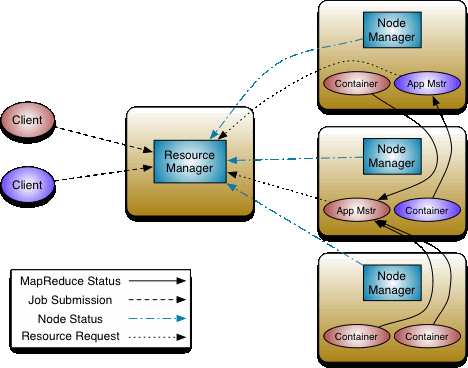
\includegraphics[width=0.5\textwidth]{Figuras/yarn.png}
    \caption{Arquitectura de YARN}
    \label{fig:yarn}
    \source{Imagen extraída de https://hadoop.apache.org/docs/r2.7.2/hadoop-yarn/hadoop-yarn-site/YARN.html}
\end{figure}


\paragraph{HDFS} \textit{Hadoop Distributed File System (HDFS)} es un sistema de archivos que abarca todos los nodos de un \textit{cluster} Hadoop para el almacenamiento de datos. Enlaza entre sí los sistemas de archivos de muchos nodos locales para convertirlos en un único gran sistema de archivos.\cite{quehadoop}

Un \textit{Cluster} HDFS esta compuesto de un \textit{NameNode},un servidor maestro que maneja el espacio de nombres del sistema de archivos y regula el acceso de los clientes a este; y un numero de \textit{DataNodes} que manejan el almacenamiento asociado a los nodos en los que son ejecutados.\cite{horhdfs}

El contenido de los archivos es dividido en grandes bloques (típicamente de 128 megabytes), y cada bloque del archivo es replicado independientemente en múltiples \textit{DataNodes}. Estos son monitoreados activamente por en \textit{NameNode}, que se encarga de replicarlo en caso de perdida.\cite{horhdfs}
El \textit{NameNode} no envía solicitudes directamente a los \textit{DataNodes}. Envia instrucciones a los \textit{DataNodes} replicando a señales enviadas periódicamente por los \textit{DataNodes}.\cite{horhdfs}

Las instrucciones incluyen comandos para: 

\begin{itemize}
    \item Replicar bloques a otros nodos.
    \item Remover copias locales de bloques.
    \item Re-registrar y enviar un reporte de bloques.
    \item Apagar el nodo.
 \end{itemize} The instructions include commands to:



\section{Spark}
Apache Spark es un motor de procesamiento de datos rápido en memoria, permite trabajar de forma eficiente con datos que requieren acceso rápido e iterativo a los conjuntos de datos.\cite{spark}

Consiste en el núcleo Spark y un conjunto de librerías. El núcleo es el métodos de ejecución distribuida, y las APIs de los lenguajes Java, Scala y Python ofrecen una plataforma para el desarrollo de aplicaciones distribuidas. Diferentes librerías adicionales desarrolladas sobre el núcleo aportan diferentes formas de trabajo para el manejo de datos. La habilidad de Spark para mantener los conuntos de datos en memoria principal a manera de cache acelera los procesos iterativos de tratamiento de datos, haciendolo ideal para la implementacion de algoritmos como los utilizados en \textit{Machine Learning}.\cite{spark}


Spark incluye la librería MLlib, la cual provee un conjunto creciente de algoritmos comúnmente usados en técnicas de ciencia de datos tales como : clasificación, regresión, filtros colaborativos, agrupamiento (\textit{clustering}), reducción de dimensionalidad.\cite{spark}

Una de las principales ventajas de Spark es su flexibilidad, puede ejecutarse junto a Hadoop a traves de  YARN y procesar data en HDFS, HBase, Cassandra, Hive, y cualquier otro formato de entrada de Hadoop.\cite{spark}

%Sección
\section{Bases de Datos}
\lhead[\thepage]{\thesection Bases de Datos}

\subsubsection{Definición}

Se puede definir una base de datos como un almacén de información actualizable de una aplicación, donde los aspectos físicos del almacenamiento y la representación de la información son transparentes al usuario. La información
almacenada en una base de datos es accesible a un nivel lógico sin necesidad de involucrar los
conceptos físicos de su complementación.\cite{6-josemy}

\subsection{Modelos de bases de datos} 

Las bases de datos pueden agruparse en modelos dependiendo de su estructura lógica y el modo como se almacenan, organizan y manipulan los datos. Se manejan principalmente dos tipos de modelos: las bases de
datos SQL y las bases de datos NoSQL.

\subsubsection{Bases de datos SQL}


Una base de datos relacional es aquella que presenta la información en tablas con filas y columnas. Una tabla es considerada como una relación, en el sentido de que es una colección de objetos de un mismo tipo (filas). Los datos en las tablas pueden estar relacionados de acuerdo a claves comunes o conceptos, y la habilidad de obtener datos relacionados de una tabla es la base del termino base de datos relacional.\cite{orcman}

La gestión de los datos, se  realiza a través de un lenguaje de consultas estructuradas (SQL), SQL permite realizar consultas interactivas con las cuales se extraerá o gestionará información de la base de datos \cite{25-carrejo}.

Algunas bases de datos relacionales conocidas son: MySQL, Oracle, PostgreSQL, MariaDB.

\subsubsection{Bases de datos NoSQL}

Con el objetivo de disminuir el acceso a la memoria secundaria del computador, hace unos años, los programadores comenzaron a utilizar distintas técnicas para almacenar los datos con mayor frecuencia de uso en la memoria RAM. Para lograr esto se basaron en un sistema donde todas las primitivas se escribían en forma clave/valor, además de las tradicionales consultas SQL en la
base de datos principal. Este enfoque les resulto de mayor comodidad a los desarrolladores, los cuales 
comenzaron a experimentar con bases de datos que utilizaban una interfaz de clave/valor para
el almacenamiento persistente, así como para la memoria caché, ya que la mayoría de sus consultas se expresaban de esa forma.\cite{dataglossary}

La interfaz de clave/valor representa la eliminación de una capa de abstracción al ser esta menos expresiva y de un nivel más bajo que un lenguaje como SQL. Estos sistemas aumenta la complejidad para el desarrollador, pero ofrecen mayor flexibilidad y control sobre el funcionamiento de la base de datos que se está manejando. También facilita a los desarrolladores de base de datos crear sistemas nuevos y experimentales para probar nuevas soluciones a requerimientos más complicados, como la escalabilidad, conjuntos de datos ampliamente distribuidos o aplicaciones de alto rendimiento.\cite{dataglossary}

En \cite{sprock}, Antonio Sprock profesor de la Universidad Central de Venezuela afirma :
\begin{quotation}
Muchos desarrolladores terminaron construyeron sus propias soluciones para almacenar datos,
y luego las publicaron como código abierto. Grandes industrias de internet, como Google,
Facebook, Twitter y Amazon han apostado a NoSQL, y defienden sus trabajos afirmando que:
no están utilizando una base de datos, sino “sistemas de almacenamiento distribuido para
gestionar datos estructurados”, se pueden ejecutar en clústers de servidores de computadoras
baratas, superan los cuellos de botella de rendimiento al manipular los grandes volúmenes de
datos, y evitan contar con mucho más de lo que puede cubrir sus necesidades. 

Por otro lado, NoSQL puede servir gran cantidad de carga de lecturas y escrituras. Implementaciones de NoSQL usadas en el mundo real incluyen los 6 TB de la base de datos del “ENSEMBLE” de la Comisión Europea usada en los modelos de comparación y calidad del aire, los nuevos 500 TB diarios de Facebook, entre sus 300 millones de nuevas fotos y los 2 billones de \textit{Likes} diarios, los 90 PB de eBay, los 51 TB de Amazon y los 2.5 PB de Walmart, entre otras.
\end{quotation}

Lo que indica que junto a Big Data, viene de la mano el auge de las bases de datos NoSQL como una forma de almacenamiento que aporta flexibilidad ante la cantidad masiva de datos que se generan hoy en día.


\subsubsection{Ventajas de bases de datos NoSQL} 
Esta forma de almacenar la información ofrece ciertas ventajas sobre los modelos relacionales. Entre las ventajas más significativas se pueden destacar:
\begin{itemize}
\item Se ejecutan en máquinas con pocos recursos.\cite{11-josemy}
\item Escalabilidad horizontal. \cite{11-josemy}
\item  Pueden manejar gran cantidad de datos, esto debido a que utilizan una estructura
distribuida.\cite{11-josemy}
\item  No genera cuellos de botella. \cite{11-josemy}
\end{itemize}
 

\subsubsection{Principales diferencias con las bases de datos SQL}
\begin{itemize}
\item  SQL no es su lenguaje principal de consultas: La mayoría de las base de datos NoSQL evitan utilizar el lenguaje SQL o lo utilizan como un lenguaje de soporte.\cite{11-josemy}
\item No utilizan estructuras fijas como tablas para el almacenamiento de los datos.\cite{11-josemy}
\item No suelen permitir operaciones JOIN: Al manejar volúmenes de datos masivos las operaciones JOIN presentan una carga muy elevada para el sistema. Esto se debe a que, cuando la operación no es la búsqueda de una clave, la sobrecarga puede llegar a ser muy costosa.\cite{11-josemy}
\item Arquitectura distribuida: La información puede estar compartida en varias máquinas mediante mecanismos de tablas \emph{hash} distribuidas. \cite{11-josemy}
\end{itemize}

\subsection{Los términos ACID y BASE}


En 1983, Andreas Reuter y Theo Härder publican el paper \emph{``Principles of Transaction-Oriented Database Recovery''} acuñando de forma oficial el termino ACID, dicho acronimo se define actualmente por los siguientes conceptos \cite{acidbase}:

\begin{itemize}
\item Atomicidad (\emph{Atomicity}): La tarea o todas las tareas en una transacción son realizadas o ninguna de ellas se realiza. Si un elemento de la transacción falla, toda la transacción lo hace.\cite{acidbase}
\item Consistencia (\emph{Consistency}): La transacción debe seguir todos los protocolos o reglas definidas por el sistema en todo momento. La transacción no viola estos protocolos y la base de datos debe permanecer en un estado consistente en el comienzo y final de una transacción, no habrá ninguna transacción a medio completar.\cite{acidbase}
\item Aislamiento (\emph{Isolation}): Ninguna transacción tendrá acceso a alguna otra que se encuentre en un estado intermedio o sin terminar. Por lo que cada transacción es independiente mientras se ejecuta.\cite{acidbase}
\item  Durabilidad (\emph{Durability}): Una vez la transacción esta completada, persistirá como completada y no puede ser deshacerse, sobrevivirá fallos en el sistema, perdida de energía y otro tipo de fallas.\cite{acidbase}
\end{itemize}
    
El concepto ACID es esencial en el ámbito de las bases de datos relacionales, sin el la fiabilidad es incierta.\cite{acidbase}


En el caso de los sistemas distribuidos que manejan grandes volumenes de datos, y deben lidiar con lo descrito en el teorema CAP, es necesario un enfoque distinto, por lo que surge BASE (\emph{Basically Available, Soft state, Eventual consistency})\cite{acidbase}:

\begin{itemize}
\item Basicamente Disponible (\emph{Basically Available}): El sistema garantiza la disponibilidad de los datos, habrá una respuesta a cualquier solicitud, pero esa respuesta puede tener fallas en obtener los datos solicitados, o, los mismos pueden contener inconsistencia o cambiado de estado.\cite{acidbase}

\item Estado suave (\emph{Soft state}: El estado del sistema puede cambiar con el tiempo, así que incluso durante tiempo sin operaciones de entrada, pueden estar sucediendo cambios debido a la consistencia eventual.\cite{acidbase} 

\item Consistencia Eventual (\emph{Eventual consistency}): El sistema sera eventualmente consistente, una vez deje de recibir operaciones de entrada.  Los datos se propagaran en todo el sistema tarde o temprano, pero el sistema continuara recibiendo operaciones de entrada y este no chequea la consistencia de cada transacción antes de moverse a la siguiente.\cite{acidbase}

\end{itemize}



\subsection{Tipos de bases de datos NoSQL}

Dependiendo de la forma en la que almacenen la información, se pueden encontrar varios tipos
distintos de bases de datos NoSQL. Los tipos más utilizados son:
\begin{itemize}

\begin{figure}[!htbp]
    \centering
    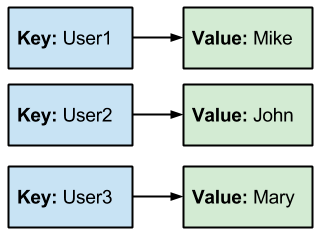
\includegraphics[width=0.5\textwidth]{Figuras/key_value.png}
    \caption{Arquitectura de base de dato Clave/Valor}
    \label{fig:arcclavevalor}
    \source{http://www.kdnuggets.com/wp-content/uploads/key-value.png}
\end{figure}

\item Bases de datos clave/valor: modelo mas utilizado entre las bases de datos NoSQL, tiene el funcionamiento mas sencillo. En este tipo de sistema, cada elemento se identifica por una clave única, lo que permite la recuperación de la información de forma rápida. Se caracterizan por ser muy eficientes tanto para las lecturas como para las escrituras.\cite{11-josemy}


\begin{figure}[!htbp]
    \centering
    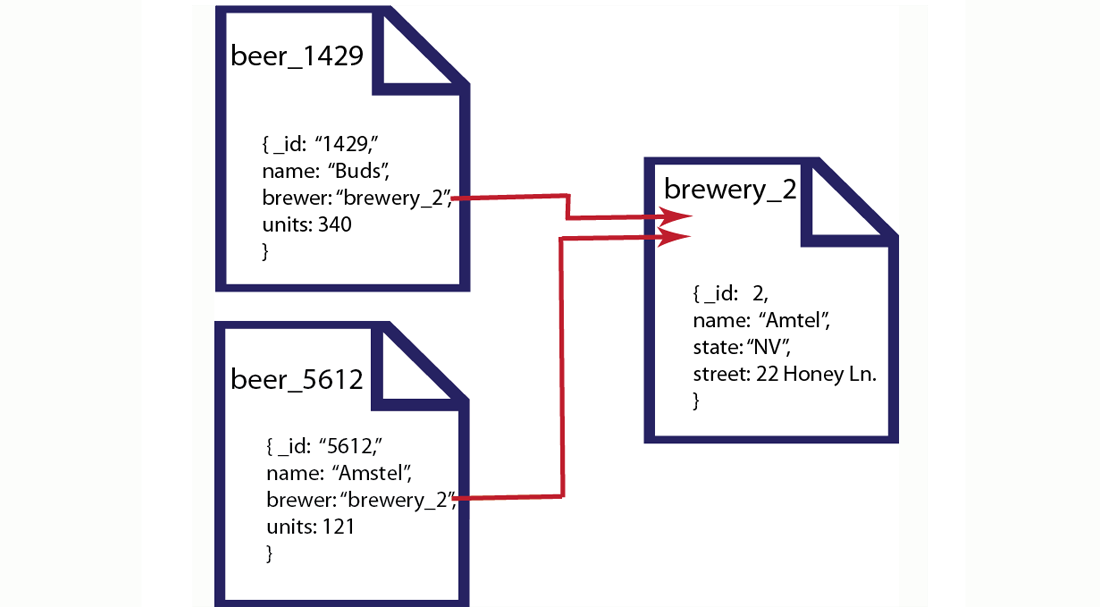
\includegraphics[width=0.8\textwidth]{Figuras/relating_docs.png}
    \caption{Arquitectura de base de dato orientada a documentos}
    \label{fig:arcdoc}
    \source{http://docs.couchbase.com/developer/dev-guide-3.0/images/relating\_docs.png}
\end{figure}

\item Bases de datos orientadas a documentos: la información es almacenada utilizando para ello una estructura simple como JSON o XML representando esta estructura al documento, cada registro es entonces asociado a un identificador único. Esta implementación permite realizar búsquedas por clave/valor y consultas avanzadas sobre el contenido del documento. Son las bases de datos NoSQL más versátiles. Se pueden utilizar en gran cantidad de proyectos, incluyendo muchos que tradicionalmente funcionarían sobre bases de datos relacionales.\cite{11-josemy}

\begin{figure}[!htbp]
    \centering
    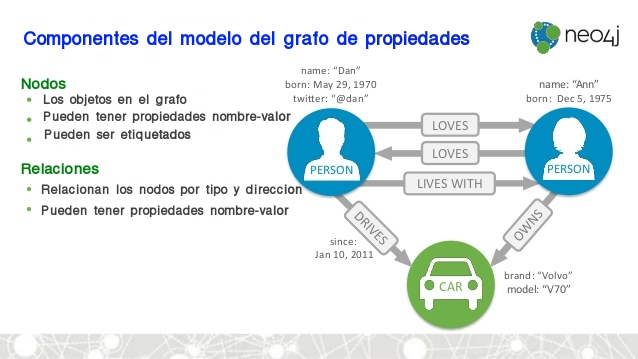
\includegraphics[width=1\textwidth]{Figuras/arcgraph.jpg}
    \caption{Arquitectura de base de dato en Grafo}
    \label{fig:arcgrpah}
    \source{http://image.slidesharecdn.com/rdbmstographsintro-150331090204-conversion-gate01/95/introduction-relational-to-graphs-13-638.jpg}
\end{figure}

\item Bases de datos en Grafo: En este tipo de bases de datos, la información se representa como nodos de un grafo y sus relaciones con las aristas del mismo, pudiendo explotarse la teoría de grafos para recorrerla \cite{11-josemy}.  A diferencia de otras bases de datos, las relaciones son la primera prioridad en las bases de datos en grafo \cite{neo4j}.

\begin{figure}[H]
    \centering
    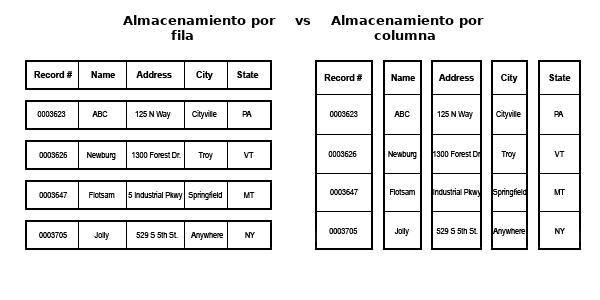
\includegraphics[width=0.7\textwidth]{Figuras/rowvcol.png}
    \caption{Base de datos tradicional vs columnar}
    \label{fig:rowvcol}
    \source{http://arxtecture.com/wp-content/uploads/2014/01/row-store-v-column-store.gif}
\end{figure}

\item Bases de datos columnares: Una base de datos columnar, también conocida como bases de datos orientadas a columnas, es una sistema manejador de base de datos que almacena los datos en columnas en vez de en filas, los datos que son almacenados aparecen en orden de guardado, lo que significa que el valor en la primera columna esta relacionado a el valor en la segunda y subsecuentes columnas si el mismo aparece en la misma fila \cite{technocolumnar}.Bajo este enfoque mejora la velocidad en recuperación de datos y operaciones que involucren los atributos de un objeto, mejorando mucho la lectura en la base de datos, sin embargo no es eficiente  al realizar escrituras a la base de datos, o cuando las operaciones involucran pocas columnas\cite{columnardb}. 


\end{itemize}

La versatilidad de las bases de datos NoSQL han originado la creacion de distintos manejadores con sus propios enfoques, la lista de bases de datos NoSQL sigue creciendo, a continuación se listan algunos de los mas utilizados:
\begin{itemize}
\item HBase : diseñado como un clon de código abierto del proyecto BigTable de Google, cuenta con una interfaz muy similar y comparten una alta compatibilidad. También utiliza un clon del sistema de archivos de Google (GFS) llamado Hadoop distributed file system (HDFS).\cite{dataglossary}

HBase está altamente integrado con el proyecto Apache Hadoop. La lectura y escritura a través de jobs MapReduce es fluida, sin embargo la latencia individual esta afectada por la carga implícita que tienen los sistemas distribuidos al lidiar con el trafico de red. El elemento fuerte de HBase se muestra cuando muchos clientes acceden de forma distribuida al sistema.\cite{dataglossary}

\item Apache Accumulo : es un almacén estructurado altamente escalable basado en BigTable de Google. Esta escrito en Java y opera sobre \emph{Hadoop Distributed File System (HDFS)}. Accumulo soporta un almacenamiento y recuperación eficiente de datos estructurados, incluidas búsquedas por rango, y provee soporte para usar las tablas de Accumulo como entras y salidas de unidades de trabajo MapReduce.\cite{manualacumulo}

Accumulo posee entre sus características balanceo de carga y particionado automático, compresión de datos y etiquetas de seguridad de grano fino.\cite{manualacumulo}

Accumulo almacena pares clave/valor ordenados. La ordenación de los datos por la clave
permite búsquedas rápidas de claves individuales o exploraciones de más de una serie de
claves. Puesto que los datos se recuperan por claves, éstas deben contener la información que
se utilizará para hacer la búsqueda. \cite{13}
El diseño original de BigTable tiene un paradigma de filas y columnas. Accumulo extiende las
columnas con una etiqueta adicional, conocida como "visibilidad", la cual proporciona el control
de acceso de grano fino.\cite{13}


\item Cassandra: Es un sistema de clave/valor distribuido, con valores muy estructurados que se realizan en una
jerarquía similar a los niveles de base de datos clásicas. Por defecto, los datos son fragmentados y equilibrados
automáticamente usando un \emph{hashing} consistente en rangos de clave, aunque permite configurar otros esquemas. \cite{dataglossary}
 Las estructuras de datos están optimizadas para un rendimiento de escritura consistente, al costo de lecturas lentas ocasionales. Una de sus características mas útil es la habilidad de especificar cuantos nodos deben aceptar antes de completas una operación de lectura o escritura. Configurar el nivel de consistencia permite ajustar las concesiones entre la disponibilidad y tolerancia a partición, para priorizas rapidez sobre consistencia o viceversa.\cite{dataglossary}

\item MongoDB: Es una base de datos orientada a documentos, con registros que son similares a objetos JSON con la habilidad de almacenar y consultar sobre atributos anidados \cite{dataglossary}.MongoDB ha sido creada para brindar escalabilidad, rendimiento y gran disponibilidad,
escalando de una implantación de servidor único a grandes arquitecturas complejas de centros multidatos. MongoDB brinda un elevado rendimiento, tanto para lectura como para escritura, potenciando la computación en memoria. La replicación nativa de MongoDB y la
tolerancia a fallos automática ofrece fiabilidad a nivel empresarial y flexibilidad operativa \cite{mongo}.

\item Redis : Dos características sobresalen en Redis: mantiene la base de datos entera en la RAM, y sus valores pueden ser estructuras de datos complejas. Aunque la estructura completa se mantiene en la RAM, es periódicamente respaldada en disco, por lo que se puede usar como una base de datos persistente. Este enfoque ofrece un rendimiento rápido y predecible, pero las velocidades caen si los datos se expanden mas allá de las capacidades de la RAM.\cite{dataglossary}

 \cite{11-josemy}
\end{itemize}


%Sección
\section{Lenguajes de Programación}
\lhead[\thepage]{\thesection Lenguajes de Programación}

\subsection{Definición}
Los lenguajes de programación son un sistema de notaciones \cite{louden-josemi20}, son utilizados en la creación de programas que controlan el comportamiento y administración de los recursos de una maquina. Usualmente son descritos con dos componentes: la sintaxis, define como sera estructurada la notación, y la semántica, que define el significado de la notación. 


\subsection{ Clasificación de los lenguajes de programación}

Los lenguajes de programación pueden agruparse de acuerdo a diferentes criterios, a continuación de describen de forma breves los mas relevantes:

\begin{itemize}
\item De acuerdo al nivel de abstracción: grado de cercanía a la forma mas básica de notación que puede ser entendida por la maquina.

  \begin{itemize}
  \item Lenguaje de Maquina: Utiliza código binario para comunicar las ordenes a la maquina, poseen un nivel de complejidad alto para su comprensión por parte de un humano.
  \item Bajo Nivel: lenguajes que presentan mayor facilidad para su comprensión y utilización que el lenguaje de maquina, son altamente dependientes de las características de la maquina donde son usados \cite{80}. 
  \item Nivel Medio: poseen un grado de abstracción mas alto pero siguen poseyendo características de los lenguajes de bajo nivel.\cite{80}
  \item Alto Nivel: son independientes de la maquina, fácil de comprender para el humano. Para su ejecución pasan por un programa interprete o compilador, que traduce las instrucciones en un lenguaje de bajo nivel.\cite{80}
  \end{itemize}
  
 \item De acuerdo a la implementación o manera de ejecutarse:
   \begin{itemize}
   \item Compilados: el programa escrito en estos lenguajes pasa por una fase de traducción o compilado, donde un programa (compilador) se encarga de llevar el lenguaje a código objeto. Luego un programa enlazador se encarga de unir el código objeto generado con las librerías necesarias para producir un programa equivalente al original pero en lenguaje de maquina \cite{81}. 
   \item Interpretados: las instrucciones de los programas escritos en este tipo de lenguajes son ejecutadas en tiempo real por otro programa conocido como interprete, que traduce las instrucciones en tiempo real para su ejecución por la maquina \cite{81}.
   \end{itemize}
   
\item De acuerdo al paradigma de programación empleado: existen lenguajes que soportan mas de un paradigma. Loa paradigmas mas comunes son:

	\begin{itemize}
	\item Imperativos: consiste de comandos explícitos y llamadas a procedimiento, llevan acabo operaciones sobre datos y modifican  los valores de las variables del programa, así como un entorno externo.\cite{dimilter}
    \item Funcionales: se basa en el uso de funciones mutuamente relacionadas. Cada función es una expresión para computar un valor y es definida como una composición de funciones estándar definidas en el lenguaje.\cite{dimilter}
    \item Lógicos: los lenguajes en este paradigma son diseñados para seguir una estructura de lógica formal, esto es, axiomas(hechos y reglas) que describen propiedades de un objeto especifico, y un teorema a ser probado.\cite{dimilter}
    \item Orientados a objeto: se describen estructuras y comportamientos de objetos y clases de objetos. Un objeto encapsula variables y funciones, mientras que las clases representan conjunto de objetos que tienen la misma estructura y comportamiento. Maneja conceptos como clases compuestas y herencia.\cite{dimilter}
	\end{itemize}
\end{itemize}

\subsection{R}

R es descrito como un lenguaje para estadística computacional. Es un proyecto GNU similar al lenguaje S, puede ser considerado como otra implementación del mismo.\cite{rproject}

El lenguaje provee  una variedad amplia de técnicas estadísticas y gráficas, y es altamente extensible gracias a la capacidad de inclusión de paquetes desarrollados por su comunidad de usuarios, en \cite{24-josemy} se puede apreciar la cantidad de funcionalidades que contiene el entorno R. Otra de las fortalezas del lenguaje se encuentra su facilidad para producir gráficas de alta calidad, incluyendo símbolos matemáticos y formulas donde se necesite.\cite{rproject}

R  esta disponible como \emph{software} libre bajos los términos de la \emph{Free Software Foundation’s GNU General Public License}.Puede ejecutarse en una gran variedad de plataformas UNIX y sistemas similares ( como \emph{FreeBSD}  y \emph{Linux}), \emph{Windows} y \emph{MacOS}.\cite{rproject}


La forma de operar de R es a través de objetos que son guardados en la memoria principal del ordenador, sin la necesidad de archivos temporales. Las operaciones de lectura y escritura de archivos se realiza para la obtención de los datos sobre los que se trabajara y el almacenamiento de resultados, la lectura puede hacerse a través de la red gracias a las funcionalidades que trae el lenguaje por defecto. El lenguaje cuenta con un gran conjunto de funciones predefinidas, y paquetes aportados por la comunidad, para su utilización por parte del usuario. Los resultados pueden ser visualizados de forma directa en la pantalla, guardarse en un objeto o escribir directamente en el disco en diferentes formatos. Los objetos resultados pueden ser analizados y modificados según la conveniencia del usuario.\cite{28-josemy}

\subsection{Java}

Lenguaje de propósito general, basado en clases, orientado a objetos. El punto fuerte de este lenguaje es su portabilidad, basado en el principio WORA (\emph{write once, run anywhere}), los programas compilados en Java pueden correr en cualquier sistema independientemente de su hardware y sistema operativo, siempre que este posea la \emph{Java Virtual Machine } (JVM), maquina virtual diseñada específicamente para la ejecución de programas de Java, sin la necesidad de que estos sean compilados nuevamente.\cite{25-josemy}

Su portabilidad y uso en el área de los dispositivos móviles (fuertemente relacionado con el sistema operativo Android) le han brindado a Java una gran popularidad. Otra característica resaltante del lenguaje en su manejo de la memoria, Java hace uso de una implementación propia de un recolector de basura
automático (\emph{Garbage Collector}), que se encarga de manejar la memoria en el ciclo de vida de un objeto. Java se define como un lenguaje para entornos de producción, no para investigaciones. \cite{25-josemy}

\subsection{Python}

Python es un lenguaje de programación de propósito general, interpretado, interactivo y orientado a objetos. Provee estructuras de datos de alto nivel, tales como listas y diccionarios, escritura dinámica, módulos, clases, excepciones, manejo automático de la memoria, entre otros. Su sintaxis es simple, manteniendo la organización en el código por medio de identación, una de sus cualidades es que reduce la complejidad en la lectura y entendimiento del código, logrado reducir los costos de mantenimiento.\cite{26-josemy,27-josemy}

Diseñado en 1990, por Guido van Rossum. El lenguaje es de licencia libre, incluso para propósitos comerciales, y puede ejecutarse en la gran mayoría de computadores modernos. \cite{26-josemy}

Python es de naturaleza modular. Su kernel puede ser extendido importando distintos módulos, trabaja con un sistema de importación fácil de utilizar por el desarrollador. Incluye una variedad de extensiones que pueden estar escritas en Python, C o C++. Los módulos o extensiones que ofrecen son muy variados y se pueden encontrar para operaciones que van desde manipulación de arreglos de caracteres, expresiones regulares, hasta Interfaces de Usuario Gráficas (GUI), utilidades para el desarrollo web, servicios del sistema operativo, paquetes para minería de datos y machine learning, entre muchos otros. \cite{26-josemy}

\subsection{Scala}

Scala es un lenguaje de programación  que guarda similitud con Java, unifica la programación orientada a objetos y la funcional\cite{scala}. Sacala es un acronimo para "lenguaje escalable " (\emph{Scalable Language}). El código generado esta a la par con el de Java y su precisión en el tipeo se traduce en la captura de problemas en tiempo de compilación y no después del despliegue \cite{scala2}.

Es puramente orientado a objetos en el sentido que cada valor es un objeto. Tipos y comportamiento de objetos son descritos por clases. Las clases pueden estar compuesta usando composiciones mixtas.\cite{scala}

Es un lenguaje funcional en el sentido de que cada función es un valor.  Anidamiento de definición de funciones y funciones de orden superior están definidas por naturaleza. Soporta una noción general de coincidencia de patrones (\emph{pattern matching}) lo cual puede modelar los tipos algebraicos usados en muchos lenguajes funcionales.\cite{scala} 








%Sección
\section{Minería de Datos}
\lhead[\thepage]{\thesection Minería de Datos}
También conocida como "Descubrimiento de conocimiento en bases de datos" (KDD por sus siglas en ingles). Se define generalmente como el proceso por el cual se descubren patrones o conocimiento relevante en fuentes de datos, p.ej., base de datos, textos, imágenes, la Web, etc. Dichos patrones deben ser validos, potencialmente útiles, y comprensibles.La minería de datos es un campo multidisciplinario que involucra  estadísticas,\emph{ machine learning}, inteligencia artificial, bases de datos, recuperación de la información, y visualización.\cite{webmining}

Son muchas las tareas involucradas en este proceso. Entre las mas comunes se tiene la clasificación, clusterización, minería por reglas de asociación, y minería por patrones secuenciales.\cite{webmining}



%--------
% Etapas del proceso KDD

% El proceso de creación de un modelo en minería de datos es un proceso cíclico, dinámico e interactivo, por lo tanto, es posible que se repita en varias ocasiones hasta obtener el modelo adecuado, sus fases suelen ser:

% 1. Definición del problema y selección del conjunto de datos: Consiste en definir el problema y los objetivos del proyecto 55. Se organiza la información disponible y la fuente de las mismas, se definen las variables objetivas e independientes y se seleccionan los registros que se encuentran disponibles para ser empleados.

% 2. Análisis de las propiedades de los datos: Consiste en explorar y revisar los datos disponibles, para luego definirlos, evaluar el valor correspondiente y verificar si están bien captados o no.

% 3. Transformación, preparación o pre procesamiento de datos: Los datos obtenidos pueden hallarse dispersos o bien estar almacenados en diversos formatos, así mismo, pueden darse casos de valores perdidos (valores incorrectos o ausentes), en esta etapa se busca depurar la base de datos eliminando aquellos que no resultan válidos, generando los faltantes y buscando correlaciones ocultas entre ellos, para de esta forma generar una estructura final compuesta de datos adecuados y precisos que faciliten su transformación y posterior análisis.

% 4. Generar modelos: Consiste en la definición de los algoritmos y técnicas de minería de datos que se van a emplear en el tratamiento de los datos, se busca obtener patrones que representen un conocimiento útil y de valor. Dichos patrones son obtenidos a través de un proceso conocido como entrenamiento, este consiste en aplicar un algoritmo a una estructura de datos para obtener patrones de ella, por tanto, dichos patrones variarán en función de los datos y el algoritmo empelado 55. Cabe acotar que en caso de que los datos cambien, será necesario cambiar el proceso de minería empleado.

% 5. Explorar y validar modelos: Consiste en la interpretación de los resultados obtenidos para determinar si las conclusiones resultan válidas y satisfactorias. En caso de que ninguno de los modelos generados funcione, el proceso puede repetirse desde el inicio o desde un paso anterior.

% 6. Implementar y actualizar modelos: En esta fase se colocan en uso los modelos que funcionen mejor para incorporarlo a los sistemas de análisis de información de la organización, dichos modelos permitirán luego generar información de utilidad para tomar decisiones de negocio.

%------------------------------------------------------
% descomentar >>>
\subsection{El proceso de la Minería de Datos}
Según \cite{webmining} una aplicación de minería de datos usualmente comienza con el entendimiento del dominio del problema por los analistas de datos, quienes luego identifican fuentes de datos adecuadas y los datos objetivo. Una vez que se obtienen los datos se comienza el proceso de minería, este generalmente se lleva acabo en 3 pasos: 
\begin{itemize}
\item Pre-procesamiento: Los datos crudos (obtenidos de la fuente sin previo procesamiento) son limpiados de ruidos y anormalidades. En muchos casos también es necesaria la reducción de estos a través de muestreo y selección de atributos o características.
\item Minería de datos: Los datos procesados son pasados a un algoritmo encargado de producir los patrones o conocimiento.
\item Post-procesamiento: En muchos casos, no todos los patrones descubiertos son útiles. Este paso identifica aquellos que tienen un valor para su aplicación. Varias evaluaciones y técnicas de visualización son utilizadas para hacer esta decisión. 
\end{itemize}

Este proceso es iterativo la mayoría de las veces . Usualmente conlleva varias rondas para alcanzar un resultado final satisfactorio, que es luego incorporado en una tarea operacional del mundo real. \cite{webmining}

\subsection{Tipos de modelo}

Los métodos y algoritmos aplicables en la minería de datos son variados, estos se definen en función de la elección del problema de estudio y los datos disponibles. A grandes rasgos, es posible identificar dos tipos de modelos:

\subsubsection{Modelos predictivos}

Como su nombre lo indica, están asociados a tareas que implican predicción, predicen el valor de un atributo o variable de interés basado en el valor de otros atributos. Dentro de este modelo, se encuentran los algoritmos de aprendizaje supervisados, en los cuales el proceso de modelaje es realizado sobre un conjunto de ejemplos formados por entradas al sistema y la respuesta que se debería dar ante cada una de ellas, de esta forma, el modelo es entrenado a través de datos para predecir una variable basada en dichos datos \cite{54}. Los modelos predictivos pueden ser de dos tipos:
 \begin{itemize}
 \item Clasificación: Dada una cantidad de registros que contienen una serie de atributos, se examinan las características de dicho registro y se le asigna una clase o categoría lo más exacta posible. En este tipo de modelos se incluyen las redes neuronales, los árboles de decisiones y el análisis discriminante.
 \item Regresión: Dada una colección de registro, se intenta predecir un valor futuro (Lo más exactamente posible) tomando como base un conjunto de valores pasados. Este modelo incluye series temporales, técnicas bayesianas, análisis de varianza y covarianza, etc.
 \end{itemize}

\subsubsection{Modelos descriptivos}

Como su nombre lo indica, se asocian a tareas descriptivas, es decir, identifican patrones o tendencias que explican o describen los datos y sus propiedades, sin tener conocimiento previo acerca de los patrones buscados. A esta categoría pertenecen los algoritmos de aprendizaje no supervisados, en donde la respuesta no está dada, sino que el proceso de modelaje se lleva a cabo únicamente sobre un registro de entradas, a partir de las cuales el sistema debe reconocer patrones para etiquetar nuevas entradas. Los modelos descriptivos pueden ser de tres tipos:

\begin{itemize}
\item Agrupación/Clustering/Segmentación: Dada una colección de registros con distintos atributos, se pretenden hallar grupos con características muy similares entre sí pero muy diferentes con respecto a los otros. No dependen de clases predefinidas.
\item Análisis de asociación: Dada una colección de registros, se busca descubrir patrones fuertemente asociados con los datos, es decir, combinaciones de atributos frecuentes que permitan establecer reglas de asociación.
\item Búsqueda de secuencias y detección de anomalías: Dada una colección de registros con una serie de atributos, se busca identificar aquellos registros cuyas características sean significativamente diferentes del resto. Este método suele ser empleado para analizar series de tiempo y detectar desviaciones significativas del comportamiento normal.
\end{itemize}

\subsection{Mineria Web}
La mineria web (\emph{Web mining}), hace referencia a la minería de datos aplicada sobre la web, su meta es la de encontrar información útil o conocimiento de la estructura de enlaces web, contenido de las paginas y uso de los datos. A diferencia de la minería de datos tradicional donde generalmente se trabaja con datos estructurados y estructuras relacionales por naturaleza, un aspecto esencial de la minería de datos web es el tener que lidiar con datos no estructurados.\cite{webmining,minwebSoumen}

Una característica que distingue a la web es la formación espontanea y evolución de clusters inducidos por tópicos y comunidades inducidas por enlaces en el grafo web. La existencia de los enlaces añaden una cantidad importante de información mas allá de la búsqueda de texto, organización por relevancia, clasificación y clusterizacion. Otra característica es que paginas HTML bien formadas representan una estructura de árbol, con texto y atributos en los nodos, esto puede revelar pistas importantes para algoritmos de minería de contenido.\cite{minwebSoumen}

Según Bing Liu (2011) las tareas de minería web pueden subdividirse basándose en el tipo de datos usados en el proceso de minería:
\begin{itemize}
\item Minería de la estructura web: descubre conocimiento útil de los enlaces (\emph{hyperlinks}) que representan la estructura de la web. Por ejemplo, de los enlaces, se pueden descubrir comunidades de usuarios que comparten un interés mutuo.
\item Minería del contenido web: extrae información útil o conocimiento del contenido de paginas web. Se puede clasificar y clusterizar paginas web en base a su tópico. En este aspecto es muy similar a la minería de datos tradicional. Sin embargo, es también posible descubrir patrones en paginas web para extraer datos útiles en base a la interacciones que tienen los usuarios con dichas paginas, como foros, redes sociales,  . Tareas que no son parte de la minería de datos tradicional.
\item Minería del uso web: se refiere al descubrimiento de patrones de acceso a las web por parte del usuario, el proceso de minería se aplica sobre web logs donde se almacena todas las acciones que lleva a cabo el usuario.
\end{itemize}

\subsection{Web Crawling y Web Scraping}

En \cite{crawlingwebCho} se define un web crawler como un programa de gran escala que recolecta decenas de miles de paginas web por segundo. Generalmente para luego almacenarlas en un repositorio local e indexarlas en base a palabras claves. Concepto similar se tiene en \cite{crawlingwebPant} donde los web crawlers se definen como programas que explotan la estructura en grafo de la web para moverse de pagina en pagina,su motivación principal es la de recuperar las paginas web y añadirlas a un repositorio local, para luego ser usadas a conveniencia por el programa.

Uno de los puntos claves para la definición de lo que es un web crawler es su capacidad para moverse en la web a través de enlaces. Y marca una diferencia importante con el concepto de Web Scraping. 

Web Scraping es el termino acuñado para la extracción de datos de una pagina web previamente encontrada por un web crawler.\cite{webscrapLawson}

\subsubsection{Infraestructura de Web Crawling}
\emph{Crawling} puede ser visto como un problema de búsqueda en un grafo. La Web es vista como un grafo de grandes proporciones con paginas como sus nodos y enlaces como sus vértices. Un \emph{crawler} empieza en alguno de los nodos del grafo (semillas) y luego sigue los vértices para alcanzar otros nodos. El proceso de obtener una pagina y extraer los enlaces es análogo a expandir un nodo en búsqueda de grafos. Un \emph{crawler} por tópico trata de seguir los vértices de los que se espera lleven a porciones del grafo que son relevantes a un tópico.\cite{crawlingwebPant} 

\begin{figure}[!htbp]
    \centering
    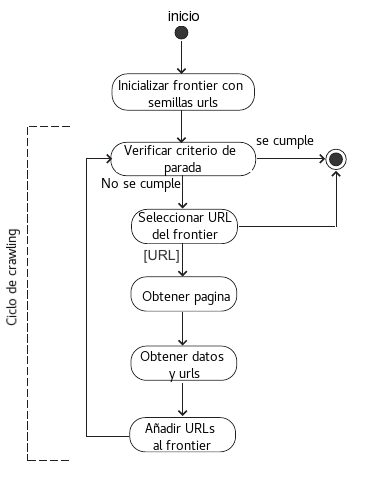
\includegraphics[width=0.5\textwidth]{Figuras/basic_sequential_crawler.png}
    \caption{Crawler basico secuencial}
    \label{fig:basiccrawler}
    \source{Imagen extraída de \cite{crawlingwebPant}}
\end{figure}


En la Figura \ref{fig:basiccrawler} se muestra el flujo básico de un \emph {crawler} secuencial. El \emph{crawler} mantiene una lista de URLs sin visitar llamada \emph{frontier}. Dicha lista es inicializada con semillas URLs (termino acuñada para referirse a URLs que inicial el proceso de \emph{crawling}). Cada iteración de \emph{crawling} involucra tomar la siguiente URL a explorar del \emph{frontier}, obtener la pagina que corresponde a la URL a traves de HTTP, extraer de esta pagina las URLs e información requerida (se podría considerar como el proceso de Webscraping), y finalmente agregar las URLs no visitadas al \emph{frontier}.

Los URLs son asignados al \emph{frontier} basándose en un puntaje previo que representa un estimado del beneficio de visitar dicha pagina.El proceso de \emph{crawling} termina cuando un numero especifico de paginas han sido exploradas. Si el \emph{frontier} esta vacío, el proceso termina de forma automática.\cite{crawlingwebPant} 
\section{Minería de Texto}
\lhead[\thepage]{\thesection Minería de Texto}

\subsection{Definición}
  En ``Untangling Text Data Mining'' , Hearst describe la minería de texto como una extensión natural de la minería de datos, cuyo objetivo principal es descubrir nuevos conocimientos e información, enfatiza la diferencia que existe entre esta y la minería de datos, en donde la búsqueda de patrones y tendencias se realiza generalmente con el objetivo de apoyar la toma de decisiones mas que el de descubrir información y conocimientos novedosos, esto ultimo lo considera algo mas propio del campo de la minería de texto. Esto se resume en la comparación hecha en el Cuadro \ref{tab:comphearst} por Hearst. \cite{untangling}
  

	 \begin{table}[ht]
      \centering\scriptsize
      \begin{tabular}{|c|c|c|c|c|c|}
       \hline 
        & Encontrando Patrones & \multicolumn{2}{ c| }{ Encontrando Nuggets}\\ \cline{1-4}
        & & Novedoso & No-Novedoso\\ \cline{1-4}
       Datos no-textuales & Mineria de datos estandar & ? & Consultas a base de datos \\ \cline{1-4}
       Datos textuales & lingüistica computacional & Minería de texto real & Recuperación de información\\ \cline{1-4}
      \end{tabular}
      \caption{Clasificación de aplicaciones de la minería de texto y minería de datos}
       \source{http://people.ischool.berkeley.edu/\~hearst/papers/acl99/acl99-tdm.html}
      \label{tab:comphearst}
  \end{table}
 

  En obras mas modernas vemos que la definición toma un aspecto general. La minería de texto puede ser definida como un proceso
  en el que un usuario interactúa con una colección de documentos usando un conjunto de herramientas de análisis, resaltando que la fuente de datos utilizada en minería de texto no son bases de datos estructuradas, sino datos textuales no estructurados en los documentos que forman parte de la colección analizada.\cite{tmhandbook}

  Puede así definirse la minería de texto como un proceso de análisis aplicado sobre datos textuales no estructurados contenidos en una colección de documentos, para el descubrimiento de información no descrita de forma explicita en los documentos analizados.

\subsection{Conceptos Básicos}

  \subsubsection{Colección de documentos}
    Cualquier agrupación de documentos de texto. Pueden ser estáticos, en cuyo caso el grupo inicial de documentos no cambia, o dinámicos termino que aplica a colecciones donde los documentos son actualizados o se agreguen nuevos documentos gradualmente.\cite{tmhandbook}

  \subsubsection{Documento}
    Puede definirse informalmente como una unidad discretas de datos textuales en una colección, que usualmente, pero no necesariamente, esta correlacionado con un documento del mundo real, como un memorandum legal, e-mail, articulo,  entre otros. Se debe resaltar que un documento no existe en una única colección, puede ser parte de cualquier numero de colecciones.\cite{tmhandbook}


  \subsubsection{Pre-procesamiento}
    Esta fase de la minería de texto (y la minería de datos) busca la conversión de los datos no estructurados y semi-estructurados a una representación estructurada como lo es un modelo vectorial. Esta fase debe llevarse acabo antes de realizar cualquier tarea de análisis o de minería de texto avanzada. Los pasos posibles de pre-procesamiento son los mismos en toda tarea de minería de texto, sin embargo cuales pasos son escogidos dependerán de la tarea a realizar.\cite{txtMiningGaryMiner}  % gary miner, practical text mining and statistical analysis for non structured text data https://books.google.co.ve/books?id=SM94BMsy50gC&printsec=frontcover&hl=es#v=onepage&q&f=false
    Los pasos básicos para el pre-procesamiento son los siguientes:
    \begin{itemize}
        \item Escoger el alcance de los textos ( \textit{Scope of documents} ): Esta etapa busca determinar si se usaran documentos completos, secciones, párrafos, u otras divisiones posibles de un documento para su posterior procesamiento usando técnicas de minería de texto. La decisión tomada dependerá del objetivo de la tarea de minería de texto, por ejemplo para tareas relacionadas con \textit{ e-mails } se escogerían los correos como el alcance, en documentos grandes esta tarea puede dificultarse, generalmente para análisis que involucren clasificación o agrupación se toma cada documento entero como el alcance.\cite{txtMiningGaryMiner}
        \item Tokenización ( \textit{Tokenization} ): Consiste en dividir las unidades de texto en palabras individuales llamadas \textit{tokens}. Esta tarea es dependiente del lenguaje en el que se encuentren los documentos, para lenguajes como el español o el ingles, una estrategia común es tomar los \textit{tokens} entre espacios o signos de puntuación, sin embargo este método debe lidiar con casos como las abreviaciones. Se puede lidiar con esta clase de inconvenientes usando métodos de tokenización inteligente que reconocen estos casos especiales.\cite{txtMiningGaryMiner}
    \item Remover palabras no informativas ( \textit{Stopping} ): en muchos casos de análisis con minería de texto es útil remover palabras comunes cuya aparición ocurre en la mayoría de textos, tales como los artículos o conectivos. Estas palabras son conocidas como \textit{stopwords} y el proceso de eliminarlas como \textit{stopping}. La remoción de estas palabras no tiene un impacto significativo en gran parte de los casos de minería de texto debido a que en los algoritmos y tecnicas usadas las \textit{stopwords} tienen poco o ningún impacto en los resultados finales. Sin embargo en casos como la recuperación de información \textit{information retrieval} el \textit{stopping} es contraproducente ya que las frases pierden su significado si algunas palabras son removidas.\cite{txtMiningGaryMiner}

    \item \textit{Stemming} y Lematización (\textit{Lemmatization}) :  \textit{stemming} es el proceso de normalizar palabras relacionadas a una misma forma. Este proceso incluye la identificación y eliminación de prefijos, sufijos y pluralizaciones inapropiadas hasta obtener un \textit{token} general que identifique todas las palabras que esten relacionadas. Como efecto de este proceso se reduce la dimensionalidad mejorando el desempeño de los algoritmos. La lematización es una forma avanzada de \textit{stemming} que intenta agrupar palabras basándose en su núcleo o lemma, el cual es determinado a partir del análisis del contexto que rodea a la palabra e información gramatical.\cite{txtMiningGaryMiner}


    \end{itemize}

  \subsubsection{Características del documento}
    La etapa de pre-procesamiento intenta aprovechar los diferentes elementos contenidos en el lenguaje natural de un documento, para transformarlo de una estructura implícita e irregular a una representación explicita. Sin embargo debido al numero de elementos que contiene un documento se debe poner especial énfasis durante el proceso de minería de datos en la identificación de un conjunto simplificado de elementos que representen al documento por completo, este conjunto de características se conoce como el modelo representativo del documento.\cite{tmhandbook}

    Debido a que los algoritmos para minería de texto operan sobre representaciones del documento basadas en características, existe una negociación entre dos metas importantes. La primera meta es representar de una forma precisa el significado del documento, lo que se traduce en un aumento de sus características representativas.
    La segunda meta es identificar las características de tal forma que sean lo mas computacionalmente eficientes y practicas para el descubrimiento de patrones, que es un proceso que busca la simplificación de los conjuntos de características.\cite{tmhandbook}

    Aunque son muchas la características que pueden representar un documento las siguientes cuatro son las mas usadas para este propósito:

    \begin{itemize}
    \item Caracteres: Los componentes individuales como letras, números, caracteres especiales y espacios son la unidad básica de construcción de características de alto nivel semántico como palabras, términos y conceptos.\cite{tmhandbook}

    \item Palabras: son el nivel básico que presenta un valor semántico. En general una característica de este nivel equivale o tiene el valor de un toquen lingüístico.  Frases, expresiones con múltiples palabras o incluso palabras unidas con guion, no constituyen características del nivel de una palabra.\cite{tmhandbook}
    \item Términos: son palabras y frases seleccionadas directamente del corpus de un documento por medio de metodologías de extracción de términos. Características de este nivel pueden estar conformadas unicamente por expresiones y palabras especificas encontradas en el documento para el que son representativas.\cite{tmhandbook}

    \item Conceptos: son características generadas para un documento por medio de metodologías de categorización manual, estadística, basa en reglas o híbridas. Pueden estar conformadas por palabras, expresiones, clausulas completas o inclusive unidades sintácticas mas grandes. Muchas de las metodologías usadas involucran un grado de referencias cruzadas con fuentes de conocimiento externo. A diferencia de las características basadas en palabras o términos, las características al nivel de conceptos pueden consistir de palabras que no estén específicamente en el documento nativo.\cite{tmhandbook}
    \end{itemize}

\subsection{TF-IDF}
  TF-IDF es un esquema de ponderación que va mas alla de evaluar si una palabra aparece o no en un documento, combina dos definiciones TF e IDF. 
  La frecuenta de términos (TF por su nombre en ingles \textit{Term Frequency}) consiste en asignar a un termino perteneciente a un documento un peso igual al numero de ocurrencias del mismo en dicho documento, se denota como $tf(t,d)$  donde $t$ representa al termino y $d$ al documento. Este método de ponderación sufre de una deficiencia, todos los términos son considerados con la misma importancia al evaluarse su relevancia para una consulta, cuando de hecho algunos términos tienen poco o ningún poder al determinar la relevancia. \cite{informationretrieval}

  IDF (por su nombre en ingles \textit{Inverse Document Frequency}) surge como una medida de contrapeso para la deficiencia de TF mencionada en el párrafo anterior. Consiste en atenuar el efecto de aquellos términos con una ocurrencia muy frecuente en la colección como para ser considerados en la determinación de la relevancia. Para este fin se denota el numero de documentos en la colección que contienen al termino $t$ como la frecuencia del documento $df_t$, y el numero total de documentos en la colección como $N$, se define entonces la frecuencia inversa del documento (idf) de un termino $t$ como sigue:
  
  \begin{equation} \label{eq:idf} 
idf_t=\log\frac{N}{df_t}
\end{equation}


  De esta forma el factor IDF es calculado con el objetivo de escalar la ponderación del termino de tal forma que el $idf$ de un termino raro es alto, mientras que el $idf$ para un termino frecuente es mas probable que sea bajo. 

  Las dos definiciones básicas TF e IDF son combinadas para producir el esquema de ponderación TF-IDF donde a cada termino $t$ le es asignado un peso en el documento $d$, esto viene dado por:
  \begin{equation} \label{eq:tfidf} 
tf\mathrm{-}idf(t,d)=tf_{t,d}\times idf_t
\end{equation}

  Esta ponderación cuenta con las siguientes características: 
  \begin{itemize}
    \item Es mayor cuando $t$ ocurre gran cantidad de veces en un numero pequeño de documentos.
    \item Menor cuando el termino ocurre pocas veces en un documento, o ocurre en muchos documentos.
    \item Mucho menor cuando el termino ocurre prácticamente en todos los documentos.
  \end{itemize}

\subsection{El modelo espacio vector y la matriz de término-documento}

  Usando el método de ponderación TF-IDF, se visualiza cada documento como un vector con una componente para cada termino contenido en la colección (este conjunto de términos es conocido como diccionario de términos, o simplemente diccionario)  junto a la ponderación dada por TF-IDF. Para términos que no ocurran en un documento su ponderación es cero.\cite{informationretrieval} 

  Esta representación del conjunto de documentos como vectores en un espacio vectorial común, es conocida como el modelo espacio vector.\cite{informationretrieval}

  Al verse un conjunto de $N$ documentos como una colección de vectores, entonces se tiene lo que es conocido como la matriz de término-documento esta es una matriz $M\times N$ cuyas filas representan los $M$ terminos de las $N$ columnas, cada una de las cuales corresponden a un documento.\cite{informationretrieval}

\subsection{Medidas de similitud entre vectores}
  Habiéndose planteado la representación de los documentos como vectores, un elemento clave para operaciones de clasificación y agrupamiento es encontrar la similitud entre dichos vectores (y por tanto entre los documentos). Con este fin se presentan las ecuaciones mas utilizadas para obtener una ponderación de la similitud:
  \subsubsection{Distancia euclídea}
    Métrica estándar para problemas geométricos, es la distancia ordinaria entre dos puntos en el espacio.
    Dados dos documentos $d_1$ y $d_2$ representados vectorialmente. La distancia euclídea entre dos documentos viene dada por:  
    \begin{equation} \label{eq:deuc} 
D(d_1,s_2)=\sqrt{\sum\limits_{i=0}^n {|d_{1,i}-d_{2,i}|}^2 }
\end{equation}

  \subsubsection{Similitud del coseno}
    Al ser representados los documentos como vectores es posible usar la correlación que existe entre ellos, siendo dos vectores $d_1$ y $d_2$ para conocer la similitud entre estos puede usarse el coseno del angulo que existe entre dicho vectores.

    Esta medida viene dada por la siguiente ecuación: 
    \begin{equation} \label{eq:cos} 
Cos(d_1,d_2)=\frac{d_1\cdot d_2}{||d_1||\cdot ||d_2||}
\end{equation}

    Donde es normalizada con la distancia euclídea ($||\cdot||_2$).

\subsection{Algoritmos de agrupación (\textit{clustering})}
  Los algoritmos de \textit{clustering} agrupan un conjunto de documento en subconjuntos o \textit{clusters}. En estos algoritmos se busca crear \textit{clusters} que posean una coherencia interna, pero estén bien diferenciados entre ellos. Son las características y distribución de los datos lo que determina la correspondencia de un documento a un grupo, no existe asignación previa de clases por lo que la agrupación es la forma mas común de aprendizaje no supervisado.
  
  
  Pueden distinguirse dos tipos de agrupamiento; agrupamiento plano (\textit{Flat clustering}), en donde el conjunto de \textit{clusters} no posee ninguna estructura explicita que relacione las agrupaciones entre ellas, agrupaciones jerárquicas (\textit{Hierarchical clustering}), en donde se crea una jerarquía entre los agrupamientos que conforman el conjunto de  \textit{clusters}.\cite{informationretrieval}
  
  El objetivo en \textit{Flat clustering} es que dado un conjunto de documentos $D = \{d_1,...,d_N\}$, el numero deseado de \textit{clusters} $K$, y una función objetivo que evalué la calidad de la asignación a las diferentes agrupaciones, se desea computar una asignación $\gamma:D\to\{1,...,K\}$ que minimice (o en otros casos maximice) la función objetivo. En la mayoría de los casos también se demanda que ninguna agrupación $K$ este vacía.\cite{informationretrieval}

  La función objetivo es generalmente definida en términos de similitud o distancia entre documentos. La selección del numero $K$ usualmente no es mas que una buena aproximación basada en experiencia o dominio de conocimiento. Sin embargo existen una serie de heuristicas que se pueden seguir para encontrar un numero adecuado de particiones, estas heuristicas se detallaran mas adelante. Otro problema que se discutirá surge de encontrar puntos de inicios adecuados, ya que si se escogen de forma desfavorable se puede perder el optimo global.\cite{informationretrieval}

    
  \subsubsection{K-medias (\textit{K-means})}
    Es uno de los algoritmos mas importantes de agrupamiento, pertenece a la categoría de agrupamiento plano, tiene como objetivo minimizar el promedio de la distancia euclídea cuadrada de documentos a partir de los centros de sus agrupaciones (\textit{clusters}), donde el centro de una agrupación se define como la media o centroide $\vec{\mu}$ de los documentos en una agrupación $\omega$: 
    \begin{equation} \label{eq:centroide} 
\vec{\mu}= \frac{1}{|\omega|}\sum_{\vec{x}\in\omega}\vec{x}
\end{equation} 
 

    Esta definición se hace en base a el modelo de espacio vector, planteado anteriormente. Una agrupación ideal en K-medias es una esfera con un centroide como su centro de gravedad. Idealmente, las agrupaciones no deben superponerse.\cite{informationretrieval}

    Una medida de evaluar que tan bien los centroides representan a los miembros de sus agrupaciones es la suma residual de cuadrados, $RSS$ (por su nombre en ingles \textit{residual sum of squares}), la distancia cuadrada de cada vector desde su centroide sumada sobre todos los vectores, esto es:
    \begin{equation} \label{eq:RSSk} 
RSS_k=\sum_{\vec{x}\in\omega_k}|\vec{x}-|\vec{\mu}(\omega_k)|^2
\end{equation}


    \begin{equation} \label{eq:RSS} 
RSS=\sum_{K=1}^k{RSS_k}
\end{equation}

    El objetivo en K-medias es minimizar a RSS.

    \begin{figure}[!htbp]
      \centering
      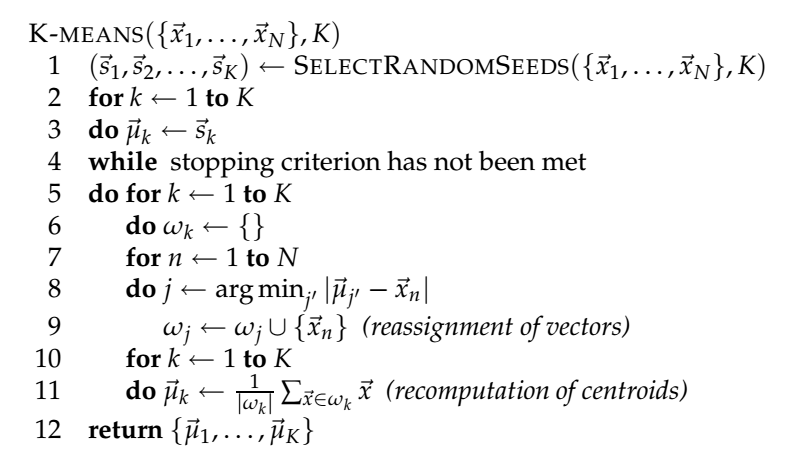
\includegraphics[width=0.7\textwidth]{Figuras/codigo_kmedias.png}
      \caption{Pseudocodigo del algoritmo de k-medias}
      \label{fig:cod_kmedias}
      \source{Imagen extraída de \cite{informationretrieval}}
   \end{figure}

    
    En base a la figura \ref{fig:cod_kmedias} se describe el algoritmo de k-medias de forma general en los siguientes pasos, se seleccionan $K$ documentos de forma aleatoria como centros iniciales de los \textit{clusters}, conocidos como semillas (\textit{seeds}). Dichos centros son transladados en el espacio, con el objetivo de minimizar RSS. Esto se hace de forma iterativa hasta cumplir con un criterio de parada, reasignando documentos al \textit{cluster} con el centroide mas cercano y recalculando cada centroide basado en los miembros actuales de su \textit{cluster}.\cite{informationretrieval}
    
    
    Los criterios de parada aplicables son:
      \begin{itemize}
        \item Un numero fijo de iteración, si bien esta condición limita el tiempo de ejecución del algoritmo puede provocar una calidad baja de agrupamiento debido a un numero insuficiente de iteraciones.
        \item La asignación de los documentos a los \textit{clusters} no cambia, exceptuando casos con malos mínimos locales. Este criterio produce una buena asignación a los \textit{clusters} pero el tiempo de ejecución podría ser excederse del rango aceptable.
        \item Los centroides no cambian entre iteraciones.
        \item Detener la ejecución del algoritmo cuando $RSS$ caiga debajo de un rango. Este criterio asegura que las agrupaciones sean de una calidad deseado al terminar el proceso. Se combina con un numero de iteraciones máximas para asegurar que la ejecución acabe.
        \item Detener la ejecución del algoritmo cuando el descenso en $RSS$ caiga debajo de un rango $\theta$. Este criterio asegura que las agrupaciones sean de una calidad deseado al terminar el proceso. Se combina con un numero de iteraciones máximas para asegurar que la ejecución acabe.
      \end{itemize}
    
    \paragraph{Cardinalidad de \textit{clusters} en K-medias}

    Seleccionar un $K$ adecuado es uno de los factores fundamentales para obtener resultados adecuados al usar K-medias, existen diferentes criterios a los que recurrir si no se puede estimar de forma previa un valor adecuado para $K$.\cite{informationretrieval}

    Un método heuristico para estimar un $K$ que minimice a $RSS$ es ejecutar $i$ agrupamientos con $K$ \textit{clusters} (cada uno con una inicialización diferente) y calcular la función $RSS$ de cada uno de estos. Luego es tomado el mínimo de los valores $RSS$ de los $i$ agrupamientos. Este mínimo es denotado como $RSS_{min}(K)$. Mientras $K$ es incrementado se inspeccionas los valores de $RSS_{min}(K)$ hasta encontrar el `codo' en la curva, este es el punto donde el decrecimiento sucesivo en $RSS_{min}(K)$ se hace notablemente pequeño. Ejemplo de esto se puede observar en la figura \ref{fig:codo} donde este efecto es notable para $K=4$  y $K=9$.\cite{informationretrieval}

    \begin{figure}[!htbp]
        \centering
        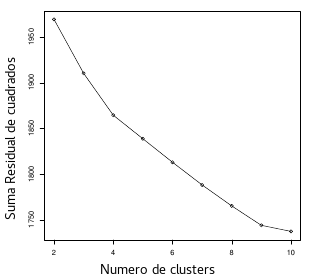
\includegraphics[width=0.7\textwidth]{Figuras/codo.png}
        \caption{Curva creada iterando valores de $K$ para la función $RSS_{min}(K)$}
        \label{fig:codo}
        \source{Imagen extraída de \cite{informationretrieval}}
      \end{figure}

    Un segundo tipo de criterio para cardinalidad de \textit{clusters} impone una penalidad por cada nuevo \textit{cluster}, conceptualmente se empieza con un unico \textit{cluster} que contiene todos los documentos y luego se busca el numero optimo de \textit{clusters} $K$ incrementando sucesivamente $K$ por uno. Esta función combina dos elementos, la distorcion que mide que tantos documentos se desvían del prototipo de sus \textit{clusters} ($RSS$ para K-medias); y una medida de complejidad de modelo. Se interpreta un agrupamiento como un modelo de los datos. La complejidad de modelo es agrupamiento es usualmente el numero de \textit{clusters} o una función para ello. Para el caso de K-medias, entonces se tiene como criterio para seleccionar $K$:
      \begin{equation} \label{eq:criterio2} 
        K = \arg_K \min[{RSS_{min}(K)+\lambda K}]
      \end{equation}

    donde $\lambda$ es un factor de ponderación. Un valor grande de $\lambda$ favorece una solución con pocos \textit{clusters}. Para $\lambda = 0$, no hay penalidad por mas \textit{clusters} y $K=N$ es la mejor solución.\cite{informationretrieval}

      


  \subsubsection{Clasificación jerárquica}
    La clasificación jerárquica no requiere la especificación de un numero de \textit{clusters} y la mayoría de los algoritmos utilizados para este tipo de clasificación son deterministicos. Estas ventajas vienen con el costo de una baja eficiencia.
    Los algoritmo de aficionan jerárquica los hay \textit{top-down}, donde requieren un método para dividir un \textit{cluster} de forma recursiva hasta que se alcancen los documentos individuales; y \textit{bottom-up}, donde cada documento es tratado como un cluster de un único elemento al principio, estos son luego mezclados (o aglomerados) en pares de forma sucesiva, este proceso se repite hasta que todos los \textit{clusters} sean mezclados en uno único que contenga todos los documentos, este algoritmo es conocido como HAC por sus siglas en ingles \textit{Hierarquical Aglomerative Clustering}.\cite{informationretrieval}   


    \paragraph{Dendogram}

      \begin{figure}[!htbp]
        \centering
        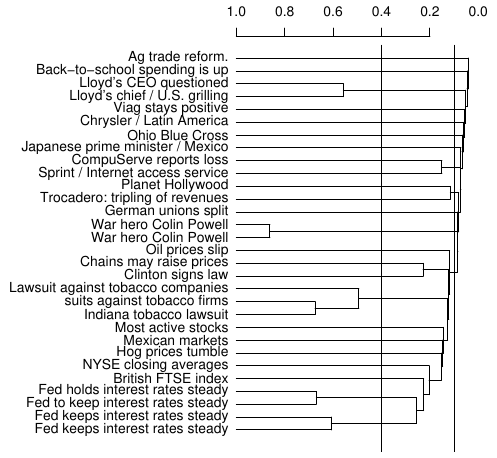
\includegraphics[width=0.7\textwidth]{Figuras/dendograma.png}
        \caption{Dendograma}
        \label{fig:dendograma}
        \source{Imagen extraída de \cite{informationretrieval}}
      \end{figure}

  

      Los agrupamientos HAC son generalmente visualizados en dendogramas, como se muestra en la figura \ref{fig:dendograma}. Cada mezcla esta representada por una linea horizontal, las coordenadas $y$ de esta linea es la similaridad de los dos \textit{clusters} que fueron unidos. Esta similitud es llamada similitud de la combinación del \textit{cluster} mezclado. El dendograma permite reconstruir la historia de las diferentes mezclas que se necesitaron para un agrupamiento especifico.\cite{informationretrieval}
    
      Para obtener un partición de \textit{clusters} diferenciados, como en el agrupamiento plano, la jerarquía debe ser cortada en algún punto. Pueden usarse diferente criterios para este fin: 

      \begin{itemize}
        \item Cortar en un nivel de similitud previamente especificado.
        \item Cortar el dendograma donde la distancia de similitud entre dos combinaciones sucesivas es mayor.
        \item  Aplicar la ecuación \ref{eq:criterio2}: 
            \begin{equation}\label{eq:criterio2.2}
               K = \arg_{K'} \min{[RSS(K')+\lambda K']}
            \end{equation} 

            Donde $K'$ se refiere al corte de la jerarquia que resulta en $K'$ \textit{clusters}, $RSS$ es la suma residual de cuadrados y $\lambda$ es una penalidad por cada \textit{cluster} adicional.
         \item También es posible especificar un numero $K$ de \textit{clusters} y seleccionar el corte que genere dicho numero.

      \end{itemize}

   


    \paragraph{Agrupamiento jerárquico simple}
      Primero se computa la matriz de similitud $C$, $N\times N$. El algoritmo luego ejecuta $N-1$ pasos de mezclar los \textit{clusters}actualmente mas similares. En cada iteración los dos \textit{clusters} mas similares son mezclados, y las filas y columnas del \textit{cluster} mezclado $i$ en $C$ son actualizadas.El agrupamiento es almacenado como una lista de mezclas en $A$. $I$ indica cuales \textit{clusters} estan disponibles para ser mezclados. La función $SIM(i,m,j)$ calcula la similaridad del cluster $j$ con la mezcla de los cluster $m$ e $i$. Este algoritmo sera refinado para las variantes de agrupamiento de enlace-individual, agrupamiento de enlace-completo, agrupamiento grupo-promedio y agrupamiento por centroide.\cite{informationretrieval}

 \begin{figure}[!htbp]
        \centering
        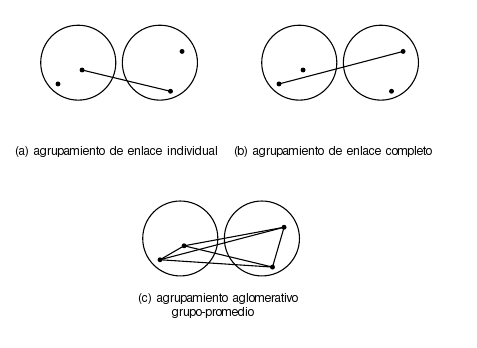
\includegraphics[width=0.7\textwidth]{Figuras/h_clust1.png}
        \caption{Tipos de agrupamientos jerarquicos}
        \label{fig:hclust}
        \source{Imagen extraída de \cite{informationretrieval}}
\end{figure}

\paragraph{Agrupamiento de enlace individual}
  En este agrupamiento la similaridad de dos \textit{clusters} es la similitud de sus miembros mas similares , ejemplo de esto se puede observar en la figura \ref{fig:hclust} (a). Este criterio es local, solo se toma en cuenta el área donde los dos \textit{clusters} están mas cercanos.\cite{informationretrieval}


\paragraph{Agrupamiento de enlace completo}

En el agrupamiento de enlace completo, la similitud de dos \textit{clusters} es la similitud de sus miembros menos similares, ejemplo en la figura \ref{fig:hclust} (b). Este criterio es no-local, la estructura completa del agrupamiento puede influenciar las decisiones al realizarse la mezcla. Esto resulta en una preferencia por \textit{clusters} compactos con diámetros pequeños, sobre \textit{clusters} largos y desordenados, sin embargo también causa sensibilidad ante valores atípicos.\cite{informationretrieval}

\paragraph{Agrupamiento aglomerativo grupo-promedio}
  El GAAC por sus siglas en ingles \textit{Group-average agglomerative clustering}, evalúa la calidad del \textit{cluster} basándose en la similitud entre todos los documentos, como se aprecia en la figura \ref{fig:hclust} (c). GAAC calcula la similitud promedio $SIM\mathrm{-}GA$ de todos los pares de documentos incluyendo pares del mismo \textit{cluster},excluyendo las similitudes de un elemento consigo mismo:

  \begin{equation}\label{eq:simga}
    SIM\mathrm{-}GA(\omega_i,\omega_j)=\frac{1}{(N_i+N_j)(N_i+N_j-1)}[(\sum_{d_m\in\omega_i\cup\omega_j}\vec{d_m})^2-(N_i+N_j)]
  \end{equation}

  donde $\vec{d}$ es la longitud normalizada del vector del documento $d$, $N_i$ y $N_j$ son el numero de documentos en $\omega_i$ y $\omega_j$, respectivamente.\cite{informationretrieval}


%En caso de una imagen colocarla de la siguiente manera
%\begin{figure}
%\centering
%\includegraphics[width=0.7\textwidth]{Figuras/nombre_de_la_figura.ext}
%\caption{\label{fig:etiqueta_de_la_figura}Titulo de la figura.}
%\end{figure}

%En caso de hacer referencia a una imagen hacerlo de la siguiente forma
%\textit{figura \ref{fig:etiqueta_de_la_figura}}

%En caso de hacer una cita y que esta se encuentre en la bibliografía
%\cite{etiqueta_de_la_referencia}


%-----------------------------------------------------------------------------
%	NOTA A LA HORA DE AGREGAR BIBLIOGRAFIAS REFERENCIAS.BIB
%-----------------------------------------------------------------------------

%ARTICLE: Un artículo de un periódico o una revista. Campos requeridos: author,title, journal, year. Campos opcionales: volume, number, pages, month, note.

%BOOK: Un libro con una editorial explícita. Campos requeridos: author o editor,title, publisher, year. Campos opcionales: volume o number, series, address,edition, month, note.

%BOOKLET: Un trabajo impreso y distribuido, pero que no tiene una editorial o institución responsable. Campos requeridos: title. Campos opcionales: author, howpublished, address, month, year, note.

%INBOOK: Una parte de un libro, como un capítulo, una sección, un rango de páginas,etc. Campos requeridos: author o editor, title, chapter o pages, publisher, year.Campos opcionales: volume o number, series, type, address, edition, month, note.

%INCOLLECTION: Una parte de un libro con título propio. Campos requeridos: author, title, booktitle, publisher, year. Campos opcionales: editor, volume o number,series, type, chapter, pages, address, edition, month, note.

%INPROCEEDINGS: Un artículo de las memorias de un congreso. Campos requeridos: author, title, booktitle, year. Campos opcionales: editor, volume o number, series, pages, address, month, organization, publisher, note. 

%MANUAL: Documentación técnica. Campos requeridos: title. Campos opcionales: author, organization, address, edition, month, year, note. 

%MASTERSTHESIS: Una tesis de maestría. Campos requeridos: author, title, school,year. Campos opcionales: type, address, month, note.

%MISC: Para cuando el resto falla. Campos requeridos: Ninguno. Campos opcionales:author, title, howpublished, month, year, note.

%PHDTHESIS: Tesis de doctorado. Campos requeridos: author, title, school, year. Campos opcionales: type, address, month, note.

%PROCEEDINGS: Las memorias de un congreso. Campos requeridos: title, year. Campos opcionales: editor, volume o number, series, address, month, organization, publisher, note.

%TECHREPORT: Un informe publicado por una institución. Campos requeridos: author,title, institution, year. Campos opcionales: type, number, address, month, note.

%UNPUBLISHED: Un documento (inédito), con un autor y un título, pero que no ha sido formalmente publicado. Campos requeridos: author, title, note. Campos opcionales: month, year.
